\documentclass[12pt]{article}
\usepackage[english]{babel}
\usepackage[utf8]{inputenc}
\usepackage[T1]{fontenc}
\usepackage{fancyhdr}
\usepackage{graphicx}
\usepackage{enumerate}
\usepackage{enumitem}
\usepackage{amsmath}
\usepackage{amssymb}
\usepackage{bm}
\usepackage{url}
\usepackage[dvipsnames]{xcolor}
\usepackage{booktabs}
\usepackage{longtable}
\usepackage{amsthm}
\usepackage[hidelinks]{hyperref}

% Formatting and Question/Answer structure adapted from the supplied template.
\setlength{\parindent}{0cm}
\addtolength{\oddsidemargin}{-2cm}
\addtolength{\evensidemargin}{-2cm}
\setlength{\textwidth}{17.78cm}
\addtolength{\topmargin}{-2.25cm}
\setlength{\textheight}{23.24cm}
\setlength{\headheight}{30pt}
\addtolength{\parskip}{5mm}
\pagestyle{fancy}

%%%%% NEW MATH DEFINITIONS %%%%%

% Mark sections of captions for referring to divisions of figures
\newcommand{\figleft}{{\em (Left)}}
\newcommand{\figcenter}{{\em (Center)}}
\newcommand{\figright}{{\em (Right)}}
\newcommand{\figtop}{{\em (Top)}}
\newcommand{\figbottom}{{\em (Bottom)}}
\newcommand{\captiona}{{\em (a)}}
\newcommand{\captionb}{{\em (b)}}
\newcommand{\captionc}{{\em (c)}}
\newcommand{\captiond}{{\em (d)}}

% Highlight a newly defined term
\newcommand{\newterm}[1]{{\bf #1}}


% Figure reference, lower-case.
\def\figref#1{figure~\ref{#1}}
% Figure reference, capital. For start of sentence
\def\Figref#1{Figure~\ref{#1}}
\def\twofigref#1#2{figures \ref{#1} and \ref{#2}}
\def\quadfigref#1#2#3#4{figures \ref{#1}, \ref{#2}, \ref{#3} and \ref{#4}}
% Section reference, lower-case.
\def\secref#1{section~\ref{#1}}
% Section reference, capital.
\def\Secref#1{Section~\ref{#1}}
% Reference to two sections.
\def\twosecrefs#1#2{sections \ref{#1} and \ref{#2}}
% Reference to three sections.
\def\secrefs#1#2#3{sections \ref{#1}, \ref{#2} and \ref{#3}}
% Reference to an equation, lower-case.
\def\eqref#1{equation~\ref{#1}}
% Reference to an equation, upper case
\def\Eqref#1{Equation~\ref{#1}}
% A raw reference to an equation---avoid using if possible
\def\plaineqref#1{\ref{#1}}
% Reference to a chapter, lower-case.
\def\chapref#1{chapter~\ref{#1}}
% Reference to an equation, upper case.
\def\Chapref#1{Chapter~\ref{#1}}
% Reference to a range of chapters
\def\rangechapref#1#2{chapters\ref{#1}--\ref{#2}}
% Reference to an algorithm, lower-case.
\def\algref#1{algorithm~\ref{#1}}
% Reference to an algorithm, upper case.
\def\Algref#1{Algorithm~\ref{#1}}
\def\twoalgref#1#2{algorithms \ref{#1} and \ref{#2}}
\def\Twoalgref#1#2{Algorithms \ref{#1} and \ref{#2}}
% Reference to a part, lower case
\def\partref#1{part~\ref{#1}}
% Reference to a part, upper case
\def\Partref#1{Part~\ref{#1}}
\def\twopartref#1#2{parts \ref{#1} and \ref{#2}}

\def\ceil#1{\lceil #1 \rceil}
\def\floor#1{\lfloor #1 \rfloor}
\def\1{\bm{1}}
\newcommand{\train}{\mathcal{D}}
\newcommand{\valid}{\mathcal{D_{\mathrm{valid}}}}
\newcommand{\test}{\mathcal{D_{\mathrm{test}}}}

\def\eps{{\epsilon}}


% Random variables
\def\reta{{\textnormal{$\eta$}}}
\def\ra{{\textnormal{a}}}
\def\rb{{\textnormal{b}}}
\def\rc{{\textnormal{c}}}
\def\rd{{\textnormal{d}}}
\def\re{{\textnormal{e}}}
\def\rf{{\textnormal{f}}}
\def\rg{{\textnormal{g}}}
\def\rh{{\textnormal{h}}}
\def\ri{{\textnormal{i}}}
\def\rj{{\textnormal{j}}}
\def\rk{{\textnormal{k}}}
\def\rl{{\textnormal{l}}}
% rm is already a command, just don't name any random variables m
\def\rn{{\textnormal{n}}}
\def\ro{{\textnormal{o}}}
\def\rp{{\textnormal{p}}}
\def\rq{{\textnormal{q}}}
\def\rr{{\textnormal{r}}}
\def\rs{{\textnormal{s}}}
\def\rt{{\textnormal{t}}}
\def\ru{{\textnormal{u}}}
\def\rv{{\textnormal{v}}}
\def\rw{{\textnormal{w}}}
\def\rx{{\textnormal{x}}}
\def\ry{{\textnormal{y}}}
\def\rz{{\textnormal{z}}}

% Random vectors
\def\rvepsilon{{\mathbf{\epsilon}}}
\def\rvtheta{{\mathbf{\theta}}}
\def\rva{{\mathbf{a}}}
\def\rvb{{\mathbf{b}}}
\def\rvc{{\mathbf{c}}}
\def\rvd{{\mathbf{d}}}
\def\rve{{\mathbf{e}}}
\def\rvf{{\mathbf{f}}}
\def\rvg{{\mathbf{g}}}
\def\rvh{{\mathbf{h}}}
\def\rvu{{\mathbf{i}}}
\def\rvj{{\mathbf{j}}}
\def\rvk{{\mathbf{k}}}
\def\rvl{{\mathbf{l}}}
\def\rvm{{\mathbf{m}}}
\def\rvn{{\mathbf{n}}}
\def\rvo{{\mathbf{o}}}
\def\rvp{{\mathbf{p}}}
\def\rvq{{\mathbf{q}}}
\def\rvr{{\mathbf{r}}}
\def\rvs{{\mathbf{s}}}
\def\rvt{{\mathbf{t}}}
\def\rvu{{\mathbf{u}}}
\def\rvv{{\mathbf{v}}}
\def\rvw{{\mathbf{w}}}
\def\rvx{{\mathbf{x}}}
\def\rvy{{\mathbf{y}}}
\def\rvz{{\mathbf{z}}}

% Elements of random vectors
\def\erva{{\textnormal{a}}}
\def\ervb{{\textnormal{b}}}
\def\ervc{{\textnormal{c}}}
\def\ervd{{\textnormal{d}}}
\def\erve{{\textnormal{e}}}
\def\ervf{{\textnormal{f}}}
\def\ervg{{\textnormal{g}}}
\def\ervh{{\textnormal{h}}}
\def\ervi{{\textnormal{i}}}
\def\ervj{{\textnormal{j}}}
\def\ervk{{\textnormal{k}}}
\def\ervl{{\textnormal{l}}}
\def\ervm{{\textnormal{m}}}
\def\ervn{{\textnormal{n}}}
\def\ervo{{\textnormal{o}}}
\def\ervp{{\textnormal{p}}}
\def\ervq{{\textnormal{q}}}
\def\ervr{{\textnormal{r}}}
\def\ervs{{\textnormal{s}}}
\def\ervt{{\textnormal{t}}}
\def\ervu{{\textnormal{u}}}
\def\ervv{{\textnormal{v}}}
\def\ervw{{\textnormal{w}}}
\def\ervx{{\textnormal{x}}}
\def\ervy{{\textnormal{y}}}
\def\ervz{{\textnormal{z}}}

% Random matrices
\def\rmA{{\mathbf{A}}}
\def\rmB{{\mathbf{B}}}
\def\rmC{{\mathbf{C}}}
\def\rmD{{\mathbf{D}}}
\def\rmE{{\mathbf{E}}}
\def\rmF{{\mathbf{F}}}
\def\rmG{{\mathbf{G}}}
\def\rmH{{\mathbf{H}}}
\def\rmI{{\mathbf{I}}}
\def\rmJ{{\mathbf{J}}}
\def\rmK{{\mathbf{K}}}
\def\rmL{{\mathbf{L}}}
\def\rmM{{\mathbf{M}}}
\def\rmN{{\mathbf{N}}}
\def\rmO{{\mathbf{O}}}
\def\rmP{{\mathbf{P}}}
\def\rmQ{{\mathbf{Q}}}
\def\rmR{{\mathbf{R}}}
\def\rmS{{\mathbf{S}}}
\def\rmT{{\mathbf{T}}}
\def\rmU{{\mathbf{U}}}
\def\rmV{{\mathbf{V}}}
\def\rmW{{\mathbf{W}}}
\def\rmX{{\mathbf{X}}}
\def\rmY{{\mathbf{Y}}}
\def\rmZ{{\mathbf{Z}}}

% Elements of random matrices
\def\ermA{{\textnormal{A}}}
\def\ermB{{\textnormal{B}}}
\def\ermC{{\textnormal{C}}}
\def\ermD{{\textnormal{D}}}
\def\ermE{{\textnormal{E}}}
\def\ermF{{\textnormal{F}}}
\def\ermG{{\textnormal{G}}}
\def\ermH{{\textnormal{H}}}
\def\ermI{{\textnormal{I}}}
\def\ermJ{{\textnormal{J}}}
\def\ermK{{\textnormal{K}}}
\def\ermL{{\textnormal{L}}}
\def\ermM{{\textnormal{M}}}
\def\ermN{{\textnormal{N}}}
\def\ermO{{\textnormal{O}}}
\def\ermP{{\textnormal{P}}}
\def\ermQ{{\textnormal{Q}}}
\def\ermR{{\textnormal{R}}}
\def\ermS{{\textnormal{S}}}
\def\ermT{{\textnormal{T}}}
\def\ermU{{\textnormal{U}}}
\def\ermV{{\textnormal{V}}}
\def\ermW{{\textnormal{W}}}
\def\ermX{{\textnormal{X}}}
\def\ermY{{\textnormal{Y}}}
\def\ermZ{{\textnormal{Z}}}

% Vectors
\def\vzero{{\bm{0}}}
\def\vone{{\bm{1}}}
\def\vmu{{\bm{\mu}}}
\def\vtheta{{\bm{\theta}}}
\def\va{{\bm{a}}}
\def\vb{{\bm{b}}}
\def\vc{{\bm{c}}}
\def\vd{{\bm{d}}}
\def\ve{{\bm{e}}}
\def\vf{{\bm{f}}}
\def\vg{{\bm{g}}}
\def\vh{{\bm{h}}}
\def\vi{{\bm{i}}}
\def\vj{{\bm{j}}}
\def\vk{{\bm{k}}}
\def\vl{{\bm{l}}}
\def\vm{{\bm{m}}}
\def\vn{{\bm{n}}}
\def\vo{{\bm{o}}}
\def\vp{{\bm{p}}}
\def\vq{{\bm{q}}}
\def\vr{{\bm{r}}}
\def\vs{{\bm{s}}}
\def\vt{{\bm{t}}}
\def\vu{{\bm{u}}}
\def\vv{{\bm{v}}}
\def\vw{{\bm{w}}}
\def\vx{{\bm{x}}}
\def\vy{{\bm{y}}}
\def\vz{{\bm{z}}}

% Elements of vectors
\def\evalpha{{\alpha}}
\def\evbeta{{\beta}}
\def\evepsilon{{\epsilon}}
\def\evlambda{{\lambda}}
\def\evomega{{\omega}}
\def\evmu{{\mu}}
\def\evpsi{{\psi}}
\def\evsigma{{\sigma}}
\def\evtheta{{\theta}}
\def\eva{{a}}
\def\evb{{b}}
\def\evc{{c}}
\def\evd{{d}}
\def\eve{{e}}
\def\evf{{f}}
\def\evg{{g}}
\def\evh{{h}}
\def\evi{{i}}
\def\evj{{j}}
\def\evk{{k}}
\def\evl{{l}}
\def\evm{{m}}
\def\evn{{n}}
\def\evo{{o}}
\def\evp{{p}}
\def\evq{{q}}
\def\evr{{r}}
\def\evs{{s}}
\def\evt{{t}}
\def\evu{{u}}
\def\evv{{v}}
\def\evw{{w}}
\def\evx{{x}}
\def\evy{{y}}
\def\evz{{z}}

% Matrix
\def\mA{{\bm{A}}}
\def\mB{{\bm{B}}}
\def\mC{{\bm{C}}}
\def\mD{{\bm{D}}}
\def\mE{{\bm{E}}}
\def\mF{{\bm{F}}}
\def\mG{{\bm{G}}}
\def\mH{{\bm{\text{\textbf{H}}}}}
\def\mI{{\bm{I}}}
\def\mJ{{\bm{J}}}
\def\mK{{\bm{K}}}
\def\mL{{\bm{L}}}
\def\mM{{\bm{M}}}
\def\mN{{\bm{N}}}
\def\mO{{\bm{O}}}
\def\mP{{\bm{P}}}
\def\mQ{{\bm{Q}}}
\def\mR{{\bm{R}}}
\def\mS{{\bm{S}}}
\def\mT{{\bm{T}}}
\def\mU{{\bm{U}}}
\def\mV{{\bm{V}}}
\def\mW{{\bm{W}}}
\def\mX{{\bm{X}}}
\def\mY{{\bm{Y}}}
\def\mZ{{\bm{Z}}}
\def\mBeta{{\bm{\beta}}}
\def\mPhi{{\bm{\Phi}}}
\def\mLambda{{\bm{\Lambda}}}
\def\mSigma{{\bm{\Sigma}}}

% Tensor
\DeclareMathAlphabet{\mathsfit}{\encodingdefault}{\sfdefault}{m}{sl}
\SetMathAlphabet{\mathsfit}{bold}{\encodingdefault}{\sfdefault}{bx}{n}
\newcommand{\tens}[1]{\bm{\mathsfit{#1}}}
\def\tA{{\tens{A}}}
\def\tB{{\tens{B}}}
\def\tC{{\tens{C}}}
\def\tD{{\tens{D}}}
\def\tE{{\tens{E}}}
\def\tF{{\tens{F}}}
\def\tG{{\tens{G}}}
\def\tH{{\tens{H}}}
\def\tI{{\tens{I}}}
\def\tJ{{\tens{J}}}
\def\tK{{\tens{K}}}
\def\tL{{\tens{L}}}
\def\tM{{\tens{M}}}
\def\tN{{\tens{N}}}
\def\tO{{\tens{O}}}
\def\tP{{\tens{P}}}
\def\tQ{{\tens{Q}}}
\def\tR{{\tens{R}}}
\def\tS{{\tens{S}}}
\def\tT{{\tens{T}}}
\def\tU{{\tens{U}}}
\def\tV{{\tens{V}}}
\def\tW{{\tens{W}}}
\def\tX{{\tens{X}}}
\def\tY{{\tens{Y}}}
\def\tZ{{\tens{Z}}}


% Graph
\def\gA{{\mathcal{A}}}
\def\gB{{\mathcal{B}}}
\def\gC{{\mathcal{C}}}
\def\gD{{\mathcal{D}}}
\def\gE{{\mathcal{E}}}
\def\gF{{\mathcal{F}}}
\def\gG{{\mathcal{G}}}
\def\gH{{\mathcal{H}}}
\def\gI{{\mathcal{I}}}
\def\gJ{{\mathcal{J}}}
\def\gK{{\mathcal{K}}}
\def\gL{{\mathcal{L}}}
\def\gM{{\mathcal{M}}}
\def\gN{{\mathcal{N}}}
\def\gO{{\mathcal{O}}}
\def\gP{{\mathcal{P}}}
\def\gQ{{\mathcal{Q}}}
\def\gR{{\mathcal{R}}}
\def\gS{{\mathcal{S}}}
\def\gT{{\mathcal{T}}}
\def\gU{{\mathcal{U}}}
\def\gV{{\mathcal{V}}}
\def\gW{{\mathcal{W}}}
\def\gX{{\mathcal{X}}}
\def\gY{{\mathcal{Y}}}
\def\gZ{{\mathcal{Z}}}

% Sets
\def\sA{{\mathbb{A}}}
\def\sB{{\mathbb{B}}}
\def\sC{{\mathbb{C}}}
\def\sD{{\mathbb{D}}}
% Don't use a set called E, because this would be the same as our symbol
% for expectation.
\def\sF{{\mathbb{F}}}
\def\sG{{\mathbb{G}}}
\def\sH{{\mathbb{H}}}
\def\sI{{\mathbb{I}}}
\def\sJ{{\mathbb{J}}}
\def\sK{{\mathbb{K}}}
\def\sL{{\mathbb{L}}}
\def\sM{{\mathbb{M}}}
\def\sN{{\mathbb{N}}}
\def\sO{{\mathbb{O}}}
\def\sP{{\mathbb{P}}}
\def\sQ{{\mathbb{Q}}}
\def\sR{{\mathbb{R}}}
\def\sS{{\mathbb{S}}}
\def\sT{{\mathbb{T}}}
\def\sU{{\mathbb{U}}}
\def\sV{{\mathbb{V}}}
\def\sW{{\mathbb{W}}}
\def\sX{{\mathbb{X}}}
\def\sY{{\mathbb{Y}}}
\def\sZ{{\mathbb{Z}}}

% Entries of a matrix
\def\emLambda{{\Lambda}}
\def\emA{{A}}
\def\emB{{B}}
\def\emC{{C}}
\def\emD{{D}}
\def\emE{{E}}
\def\emF{{F}}
\def\emG{{G}}
\def\emH{{H}}
\def\emI{{I}}
\def\emJ{{J}}
\def\emK{{K}}
\def\emL{{L}}
\def\emM{{M}}
\def\emN{{N}}
\def\emO{{O}}
\def\emP{{P}}
\def\emQ{{Q}}
\def\emR{{R}}
\def\emS{{S}}
\def\emT{{T}}
\def\emU{{U}}
\def\emV{{V}}
\def\emW{{W}}
\def\emX{{X}}
\def\emY{{Y}}
\def\emZ{{Z}}
\def\emSigma{{\Sigma}}

% entries of a tensor
% Same font as tensor, without \bm wrapper
\newcommand{\etens}[1]{\mathsfit{#1}}
\def\etLambda{{\etens{\Lambda}}}
\def\etA{{\etens{A}}}
\def\etB{{\etens{B}}}
\def\etC{{\etens{C}}}
\def\etD{{\etens{D}}}
\def\etE{{\etens{E}}}
\def\etF{{\etens{F}}}
\def\etG{{\etens{G}}}
\def\etH{{\etens{H}}}
\def\etI{{\etens{I}}}
\def\etJ{{\etens{J}}}
\def\etK{{\etens{K}}}
\def\etL{{\etens{L}}}
\def\etM{{\etens{M}}}
\def\etN{{\etens{N}}}
\def\etO{{\etens{O}}}
\def\etP{{\etens{P}}}
\def\etQ{{\etens{Q}}}
\def\etR{{\etens{R}}}
\def\etS{{\etens{S}}}
\def\etT{{\etens{T}}}
\def\etU{{\etens{U}}}
\def\etV{{\etens{V}}}
\def\etW{{\etens{W}}}
\def\etX{{\etens{X}}}
\def\etY{{\etens{Y}}}
\def\etZ{{\etens{Z}}}

% The true underlying data generating distribution
\newcommand{\pdata}{p_{\rm{data}}}
% The empirical distribution defined by the training set
\newcommand{\ptrain}{\hat{p}_{\rm{data}}}
\newcommand{\Ptrain}{\hat{P}_{\rm{data}}}
% The model distribution
\newcommand{\pmodel}{p_{\rm{model}}}
\newcommand{\Pmodel}{P_{\rm{model}}}
\newcommand{\ptildemodel}{\tilde{p}_{\rm{model}}}
% Stochastic autoencoder distributions
\newcommand{\pencode}{p_{\rm{encoder}}}
\newcommand{\pdecode}{p_{\rm{decoder}}}
\newcommand{\precons}{p_{\rm{reconstruct}}}

\newcommand{\laplace}{\mathrm{Laplace}} % Laplace distribution

\newcommand{\E}{\mathbb{E}}
\newcommand{\Ls}{\mathcal{L}}
\newcommand{\R}{\mathbb{R}}
\newcommand{\emp}{\tilde{p}}
\newcommand{\lr}{\alpha}
\newcommand{\reg}{\lambda}
\newcommand{\rect}{\mathrm{rectifier}}
\newcommand{\softmax}{\mathrm{softmax}}
\newcommand{\sigmoid}{\sigma}
\newcommand{\softplus}{\zeta}
\newcommand{\KL}{D_{\mathrm{KL}}}
\newcommand{\Var}{\mathrm{Var}}
\newcommand{\standarderror}{\mathrm{SE}}
\newcommand{\Cov}{\mathrm{Cov}}
% Wolfram Mathworld says $L^2$ is for function spaces and $\ell^2$ is for vectors
% But then they seem to use $L^2$ for vectors throughout the site, and so does
% wikipedia.
\newcommand{\normlzero}{L^0}
\newcommand{\normlone}{L^1}
\newcommand{\normltwo}{L^2}
\newcommand{\normlp}{L^p}
\newcommand{\normmax}{L^\infty}

\newcommand{\parents}{Pa} % See usage in notation.tex. Chosen to match Daphne's book.

\DeclareMathOperator*{\argmax}{arg\,max}
\DeclareMathOperator*{\argmin}{arg\,min}

\DeclareMathOperator{\sign}{sign}
\DeclareMathOperator{\Tr}{Tr}
\let\ab\allowbreak


%%% new
\newcommand{\diag}{\mathop{\mathrm{diag}}\nolimits}
\usepackage{cancel}
\newcommand{\ttt}[1]{\texttt{#1}}

\newif\ifexercise
\exercisetrue
\newif\ifsolution
\solutiontrue

\theoremstyle{definition}
\newtheorem{exercise}{Question}
\newtheorem{answer}{Answer}
\newcommand{\Exercise}[1]{\ifexercise#1\fi}
\definecolor{answer}{rgb}{0.00, 0.12, 0.60}
\newcommand{\Answer}[1]{%
  \ifsolution
    \begingroup
    \color{answer}
    \begin{answer}#1\end{answer}
    \endgroup
  \fi
}
\setlist[enumerate,1]{leftmargin=*, label=\arabic*.}

% Replace placeholders with your own text and actual experimental outputs.
% No experimental results, parameter counts, or interpretations are filled in.
\newcommand{\ToComplete}{\textit{[To be completed.]}}
\newcommand{\Blank}{\textemdash}
\newcommand{\FigurePlaceholder}[1]{%
  \par\smallskip
  \noindent\fbox{\parbox[c][2.2cm][c]{0.94\linewidth}{\centering\itshape #1}}
  \par\smallskip
}
% Optional: put exported figures in a report-assets/ directory beside this file.
\graphicspath{{report-assets/}}
\newcounter{qfig}
\newcommand{\PlotFigure}[3]{%
  \par\medskip\noindent
  \begin{minipage}{\linewidth}\centering
  \includegraphics[width=\linewidth]{#1}\par\smallskip
  {\small\refstepcounter{qfig}\label{#2}\textbf{Figure~\theqfig.} #3\par}
  \end{minipage}\par\medskip}

\begin{document}

\fancyhead{}
\fancyfoot{}
\fancyhead[L]{\begin{tabular}[b]{l}
  IFT6135-A2026 \\
  Prof: Aishwarya Agrawal
\end{tabular}}
\fancyhead[R]{\begin{tabular}[b]{r}
  Assignment 1 -- Programming Report \\
  Multilayer Perceptrons and Convolutional Neural Networks
\end{tabular}}
\fancyfoot[C]{\thepage\quad -- Do not distribute --}

\textbf{Due Date: October 13th, 2026 at 11:00 pm}

\textbf{Student name:} Marsel Bakashov\par
\textbf{Student number:} 20216284\par
\textbf{Q1 Google Colab notebook (executed, publicly accessible):} \url{https://colab.research.google.com/drive/1K38tKGNHuw3NXDRJkKhooKXgUuytqIHL?usp=sharing}\par
\textbf{Q2 Google Colab notebook (executed, publicly accessible):} \url{https://colab.research.google.com/drive/1fTRXwrE2kt9Gz6Kp0baYwhKeMgoXxcaP?usp=sharing}\par

% These are the written-report questions only. The original handout is unchanged.
% Select the appropriate answer pages for each question on Gradescope.

\begin{exercise}[20] \textbf{(MLP Implementation with NumPy)}
\Exercise{
\subsection*{Part 2: Time Series Forecasting -- Evaluation and Analysis}

\begin{enumerate}[label=\textbf{1.2.\arabic*}, leftmargin=*]

\item \textbf{(3 points)} For every combination of dataset, model, and (context, horizon) setting, report the test
\texttt{MSE} and test \texttt{MAE}.

For the noisy datasets, you have access to both the noisy targets and the underlying
noiseless ground truth. In addition to the metrics above, compute \texttt{gt\_test\_mse} and
\texttt{gt\_test\_mae}: the MSE and MAE of each model's predictions evaluated against the
\emph{noiseless} ground truth, rather than the noisy targets. These metrics measure how well
a model recovers the true underlying signal, i.e.\ how good a denoiser it is.

\item \textbf{(3 points)} Using \texttt{gt\_test\_mse} and \texttt{gt\_test\_mae}, identify the best- and worst-performing models on each dataset and plot their predictions. Are these results consistent with what you would expect based on the depth and choice of activation function of each model?

\item \textbf{(3 points)}
For tasks with a prediction horizon of $p=336$, both 96-step and 336-step contexts are available. Report the number of cases in which each context yields the best prediction. Are these results consistent with your initial expectations?

\end{enumerate}
}
\end{exercise}

\clearpage
\Answer{
\leavevmode\par
\begin{enumerate}[label=\textbf{1.2.\arabic*}, leftmargin=*]

\item \textbf{Test metrics.}\par
\textbf{AI assistance.} Tables~\ref{tab:q1-test-metrics} and~\ref{tab:q1-gt-metrics} were completed with the help of an AI assistant, which took the values directly from the \texttt{results/results.csv} file produced by \texttt{train.py} (default settings, 300 experiments).

{% Tables generated from results/results.csv (output of train.py with its default settings).
% Values are rounded to 3 significant digits; ground-truth columns exist for the noisy datasets only.
\scriptsize
\setlength{\tabcolsep}{2.4pt}
\setlength{\LTleft}{0pt}
\setlength{\LTright}{0pt plus 1fill}
\setlength{\LTcapwidth}{0.9\linewidth}
\begin{longtable}{@{}llc@{\hspace{6pt}}rr@{\hspace{8pt}}rr@{\hspace{8pt}}rr@{\hspace{8pt}}rr@{\hspace{8pt}}rr@{}}
\caption{Test MSE and MAE of the five models for every dataset and $(h,p)$ setting (300 experiments). $h$ is the context length and $p$ the prediction horizon; SNR is the signal-to-noise ratio of the noisy datasets (clean: noiseless). \texttt{MLP\_1} is the 1-layer MLP; \texttt{MLP\_2\_ReLU} and \texttt{MLP\_2\_Tanh} are 2-layer MLPs with that hidden activation, trained with MSE; \texttt{MLP\_2\_Sig\_MSE} and \texttt{MLP\_2\_Sig\_MAE} use a sigmoid hidden activation and are trained with MSE and MAE, respectively. Errors are computed on the original (non-standardized) scale and rounded to 3 significant digits.}\label{tab:q1-test-metrics}\\
\toprule
Dataset & SNR & $(h,p)$ & \multicolumn{2}{c}{\texttt{MLP\_1}} & \multicolumn{2}{c}{\texttt{MLP\_2\_ReLU}} & \multicolumn{2}{c}{\texttt{MLP\_2\_Sig\_MSE}} & \multicolumn{2}{c}{\texttt{MLP\_2\_Sig\_MAE}} & \multicolumn{2}{c}{\texttt{MLP\_2\_Tanh}} \\
\cmidrule(lr){4-5}\cmidrule(lr){6-7}\cmidrule(lr){8-9}\cmidrule(lr){10-11}\cmidrule(lr){12-13}
 & (dB) &  & MSE & MAE & MSE & MAE & MSE & MAE & MSE & MAE & MSE & MAE \\
\midrule
\endfirsthead
\toprule
Dataset & SNR & $(h,p)$ & \multicolumn{2}{c}{\texttt{MLP\_1}} & \multicolumn{2}{c}{\texttt{MLP\_2\_ReLU}} & \multicolumn{2}{c}{\texttt{MLP\_2\_Sig\_MSE}} & \multicolumn{2}{c}{\texttt{MLP\_2\_Sig\_MAE}} & \multicolumn{2}{c}{\texttt{MLP\_2\_Tanh}} \\
\cmidrule(lr){4-5}\cmidrule(lr){6-7}\cmidrule(lr){8-9}\cmidrule(lr){10-11}\cmidrule(lr){12-13}
 & (dB) &  & MSE & MAE & MSE & MAE & MSE & MAE & MSE & MAE & MSE & MAE \\
\midrule
\endhead
\midrule
\multicolumn{13}{r}{\textit{Continued on the next page.}} \\
\endfoot
\bottomrule
\endlastfoot
\texttt{sine\_slow} & clean & 96/336 & 7.2e\textminus 9 & 6.96e\textminus 5 & 0.00396 & 0.0501 & 0.0777 & 0.246 & 0.235 & 0.423 & 0.00302 & 0.0438 \\
 &  & 336/336 & 2.41e\textminus 9 & 3.98e\textminus 5 & 0.00348 & 0.0473 & 0.0585 & 0.212 & 0.177 & 0.358 & 0.00337 & 0.0461 \\
 &  & 336/720 & 2.02e\textminus 9 & 3.73e\textminus 5 & 0.00657 & 0.0647 & 0.219 & 0.417 & 0.378 & 0.546 & 0.0116 & 0.0883 \\
\addlinespace[2pt]
 & 20 & 96/336 & 0.00728 & 0.068 & 0.0101 & 0.0801 & 0.0836 & 0.251 & 0.242 & 0.427 & 0.00853 & 0.0736 \\
 &  & 336/336 & 0.00992 & 0.0794 & 0.00978 & 0.0788 & 0.0638 & 0.217 & 0.184 & 0.363 & 0.0089 & 0.0751 \\
 &  & 336/720 & 0.00804 & 0.0715 & 0.0123 & 0.0883 & 0.224 & 0.419 & 0.383 & 0.547 & 0.0165 & 0.104 \\
\addlinespace[2pt]
 & 0 & 96/336 & 0.675 & 0.656 & 0.577 & 0.606 & 0.693 & 0.669 & 0.88 & 0.761 & 0.531 & 0.582 \\
 &  & 336/336 & 0.891 & 0.753 & 0.59 & 0.614 & 0.619 & 0.63 & 0.831 & 0.736 & 0.525 & 0.579 \\
 &  & 336/720 & 0.785 & 0.706 & 0.578 & 0.606 & 0.819 & 0.73 & 0.949 & 0.791 & 0.536 & 0.585 \\
\addlinespace[2pt]
 & $-10$ & 96/336 & 6.46 & 2.02 & 5.59 & 1.88 & 5.35 & 1.84 & 5.4 & 1.85 & 5.55 & 1.87 \\
 &  & 336/336 & 8.3 & 2.3 & 5.79 & 1.92 & 5.43 & 1.85 & 5.49 & 1.86 & 5.64 & 1.89 \\
 &  & 336/720 & 7.67 & 2.21 & 5.74 & 1.91 & 5.48 & 1.86 & 5.55 & 1.88 & 5.67 & 1.9 \\
\midrule
\texttt{sine\_fast} & clean & 96/336 & 2.81e\textminus 9 & 4.1e\textminus 5 & 0.00461 & 0.0544 & 0.0821 & 0.252 & 0.251 & 0.437 & 0.00281 & 0.0424 \\
 &  & 336/336 & 2.12e\textminus 9 & 3.69e\textminus 5 & 0.00324 & 0.0458 & 0.0633 & 0.22 & 0.193 & 0.373 & 0.00356 & 0.0476 \\
 &  & 336/720 & 3.67e\textminus 10 & 1.58e\textminus 5 & 0.00654 & 0.0647 & 0.224 & 0.422 & 0.385 & 0.549 & 0.0114 & 0.088 \\
\addlinespace[2pt]
 & 20 & 96/336 & 0.00796 & 0.071 & 0.0112 & 0.0845 & 0.0885 & 0.258 & 0.256 & 0.441 & 0.00874 & 0.0744 \\
 &  & 336/336 & 0.0107 & 0.0823 & 0.00978 & 0.0788 & 0.0692 & 0.226 & 0.199 & 0.379 & 0.00953 & 0.0777 \\
 &  & 336/720 & 0.00867 & 0.0742 & 0.0126 & 0.0896 & 0.232 & 0.427 & 0.392 & 0.554 & 0.017 & 0.105 \\
\addlinespace[2pt]
 & 0 & 96/336 & 0.661 & 0.647 & 0.564 & 0.597 & 0.696 & 0.667 & 0.886 & 0.761 & 0.52 & 0.573 \\
 &  & 336/336 & 0.874 & 0.744 & 0.574 & 0.601 & 0.616 & 0.622 & 0.836 & 0.734 & 0.512 & 0.567 \\
 &  & 336/720 & 0.763 & 0.695 & 0.56 & 0.593 & 0.821 & 0.727 & 0.956 & 0.791 & 0.516 & 0.568 \\
\addlinespace[2pt]
 & $-10$ & 96/336 & 6.41 & 2.02 & 5.6 & 1.88 & 5.37 & 1.84 & 5.43 & 1.85 & 5.58 & 1.88 \\
 &  & 336/336 & 8.11 & 2.27 & 5.69 & 1.9 & 5.35 & 1.84 & 5.43 & 1.86 & 5.49 & 1.87 \\
 &  & 336/720 & 7.46 & 2.18 & 5.62 & 1.88 & 5.36 & 1.84 & 5.43 & 1.85 & 5.54 & 1.87 \\
\midrule
\texttt{linear\_trend} & clean & 96/336 & 6.72e6 & 2.36e3 & 2.02e7 & 3.94e3 & 2.23e9 & 4.69e4 & 2.56e9 & 5.01e4 & 1.58e9 & 3.93e4 \\
 &  & 336/336 & 1.18e7 & 3.18e3 & 4.89e7 & 6.54e3 & 2.39e9 & 4.86e4 & 2.61e9 & 5.08e4 & 1.7e9 & 4.09e4 \\
 &  & 336/720 & 8.11e7 & 8.31e3 & 2.16e8 & 1.35e4 & 3.09e9 & 5.54e4 & 3.63e9 & 5.99e4 & 2.31e9 & 4.79e4 \\
\addlinespace[2pt]
 & 20 & 96/336 & 2.08e7 & 3.67e3 & 3.25e7 & 4.7e3 & 2.26e9 & 4.71e4 & 2.68e9 & 5.12e4 & 1.62e9 & 3.98e4 \\
 &  & 336/336 & 3.16e7 & 4.55e3 & 6.21e7 & 6.84e3 & 2.41e9 & 4.88e4 & 2.72e9 & 5.17e4 & 1.76e9 & 4.16e4 \\
 &  & 336/720 & 9.81e7 & 8.62e3 & 2.26e8 & 1.34e4 & 3.12e9 & 5.56e4 & 3.69e9 & 6.04e4 & 2.34e9 & 4.81e4 \\
\addlinespace[2pt]
 & 0 & 96/336 & 1.34e9 & 2.94e4 & 1.24e9 & 2.83e4 & 3.89e9 & 5.44e4 & 4.89e9 & 6.24e4 & 2.6e9 & 4.27e4 \\
 &  & 336/336 & 1.71e9 & 3.31e4 & 1.25e9 & 2.85e4 & 3.77e9 & 5.33e4 & 4.81e9 & 6.18e4 & 3.02e9 & 4.67e4 \\
 &  & 336/720 & 1.61e9 & 3.21e4 & 1.55e9 & 3.16e4 & 4.71e9 & 6.12e4 & 5.26e9 & 6.54e4 & 3.32e9 & 4.95e4 \\
\addlinespace[2pt]
 & $-10$ & 96/336 & 1.4e10 & 9.47e4 & 1.39e10 & 9.52e4 & 1.39e10 & 9.55e4 & 1.42e10 & 9.66e4 & 1.31e10 & 9.23e4 \\
 &  & 336/336 & 1.62e10 & 1.02e5 & 1.37e10 & 9.43e4 & 1.37e10 & 9.5e4 & 1.41e10 & 9.64e4 & 1.28e10 & 9.1e4 \\
 &  & 336/720 & 1.59e10 & 1.01e5 & 1.42e10 & 9.61e4 & 1.38e10 & 9.53e4 & 1.41e10 & 9.63e4 & 1.4e10 & 9.56e4 \\
\midrule
\texttt{quadra\_trend} & clean & 96/336 & 1.01e11 & 2.46e5 & 6.51e13 & 7.1e6 & 5.12e15 & 7.08e7 & 5.94e15 & 7.63e7 & 4.39e15 & 6.54e7 \\
 &  & 336/336 & 1.65e11 & 3.15e5 & 1.46e14 & 1.13e7 & 5.45e15 & 7.32e7 & 6.18e15 & 7.8e7 & 4.63e15 & 6.74e7 \\
 &  & 336/720 & 3.76e13 & 5.57e6 & 6.97e14 & 2.4e7 & 6.34e15 & 7.93e7 & 7.13e15 & 8.4e7 & 5.41e15 & 7.32e7 \\
\addlinespace[2pt]
 & 20 & 96/336 & 1.91e13 & 3.48e6 & 8.47e13 & 7.73e6 & 5.19e15 & 7.12e7 & 6.14e15 & 7.75e7 & 4.53e15 & 6.64e7 \\
 &  & 336/336 & 2.63e13 & 4.08e6 & 1.83e14 & 1.21e7 & 5.49e15 & 7.35e7 & 6.36e15 & 7.91e7 & 4.79e15 & 6.85e7 \\
 &  & 336/720 & 6.03e13 & 6.44e6 & 7.93e14 & 2.54e7 & 6.42e15 & 7.97e7 & 7.21e15 & 8.44e7 & 5.52e15 & 7.38e7 \\
\addlinespace[2pt]
 & 0 & 96/336 & 2.06e15 & 3.63e7 & 3.84e15 & 5.02e7 & 7.96e15 & 8.11e7 & 8.51e15 & 8.43e7 & 5.5e15 & 6.49e7 \\
 &  & 336/336 & 2.27e15 & 3.8e7 & 2.31e15 & 3.84e7 & 8.07e15 & 8.18e7 & 8.73e15 & 8.56e7 & 6.12e15 & 6.93e7 \\
 &  & 336/720 & 2.42e15 & 3.92e7 & 5.6e15 & 6.2e7 & 8.82e15 & 8.64e7 & 9.06e15 & 8.77e7 & 7.4e15 & 7.75e7 \\
\addlinespace[2pt]
 & $-10$ & 96/336 & 2.39e16 & 1.24e8 & 2.1e16 & 1.17e8 & 2.04e16 & 1.15e8 & 2.08e16 & 1.16e8 & 2.09e16 & 1.16e8 \\
 &  & 336/336 & 2.59e16 & 1.28e8 & 2.14e16 & 1.17e8 & 2.05e16 & 1.15e8 & 2.08e16 & 1.16e8 & 2.12e16 & 1.17e8 \\
 &  & 336/720 & 2.67e16 & 1.31e8 & 2.14e16 & 1.18e8 & 2.05e16 & 1.15e8 & 2.09e16 & 1.16e8 & 2.13e16 & 1.17e8 \\
\midrule
\texttt{expo\_trend} & clean & 96/336 & 1.33e6 & 933 & 6.54e6 & 2.03e3 & 7.04e8 & 2.36e4 & 7.09e8 & 2.37e4 & 6.98e8 & 2.35e4 \\
 &  & 336/336 & 3.22e6 & 1.52e3 & 1.55e7 & 3.35e3 & 7.99e8 & 2.58e4 & 8.05e8 & 2.59e4 & 7.93e8 & 2.57e4 \\
 &  & 336/720 & 6.62e7 & 6.91e3 & 1.05e8 & 8.62e3 & 7.37e8 & 2.53e4 & 7.4e8 & 2.53e4 & 7.33e8 & 2.52e4 \\
\addlinespace[2pt]
 & 20 & 96/336 & 6.81e8 & 2.14e4 & 7.03e8 & 2.28e4 & 7.1e8 & 2.37e4 & 7.11e8 & 2.37e4 & 7.06e8 & 2.36e4 \\
 &  & 336/336 & 4.68e8 & 1.74e4 & 7.47e8 & 2.34e4 & 8.07e8 & 2.59e4 & 8.07e8 & 2.59e4 & 8.02e8 & 2.58e4 \\
 &  & 336/720 & 6.95e8 & 2.28e4 & 7.66e8 & 2.51e4 & 7.4e8 & 2.53e4 & 7.4e8 & 2.53e4 & 7.39e8 & 2.52e4 \\
\addlinespace[2pt]
 & 0 & 96/336 & 1.08e9 & 2.64e4 & 8.82e8 & 2.45e4 & 8.45e8 & 2.44e4 & 8.48e8 & 2.44e4 & 8.51e8 & 2.44e4 \\
 &  & 336/336 & 1.3e9 & 2.86e4 & 9.83e8 & 2.62e4 & 9.42e8 & 2.63e4 & 9.45e8 & 2.64e4 & 9.51e8 & 2.63e4 \\
 &  & 336/720 & 1.05e9 & 2.67e4 & 9.07e8 & 2.58e4 & 8.81e8 & 2.57e4 & 8.82e8 & 2.57e4 & 8.92e8 & 2.57e4 \\
\addlinespace[2pt]
 & $-10$ & 96/336 & 2.53e9 & 4e4 & 2.09e9 & 3.64e4 & 1.99e9 & 3.56e4 & 2.01e9 & 3.57e4 & 2.11e9 & 3.66e4 \\
 &  & 336/336 & 3.19e9 & 4.48e4 & 2.23e9 & 3.76e4 & 2.1e9 & 3.66e4 & 2.11e9 & 3.66e4 & 2.24e9 & 3.78e4 \\
 &  & 336/720 & 2.75e9 & 4.18e4 & 2.1e9 & 3.66e4 & 2.02e9 & 3.59e4 & 2.03e9 & 3.6e4 & 2.11e9 & 3.67e4 \\
\end{longtable}

\medskip
\begin{longtable}{@{}llc@{\hspace{6pt}}rr@{\hspace{8pt}}rr@{\hspace{8pt}}rr@{\hspace{8pt}}rr@{\hspace{8pt}}rr@{}}
\caption{Ground-truth errors \texttt{gt\_test\_mse} and \texttt{gt\_test\_mae} (predictions against the noiseless series) for the 225 experiments on the noisy datasets; same layout and model names as Table~\ref{tab:q1-test-metrics}. These metrics are not computed for the clean datasets.}\label{tab:q1-gt-metrics}\\
\toprule
Dataset & SNR & $(h,p)$ & \multicolumn{2}{c}{\texttt{MLP\_1}} & \multicolumn{2}{c}{\texttt{MLP\_2\_ReLU}} & \multicolumn{2}{c}{\texttt{MLP\_2\_Sig\_MSE}} & \multicolumn{2}{c}{\texttt{MLP\_2\_Sig\_MAE}} & \multicolumn{2}{c}{\texttt{MLP\_2\_Tanh}} \\
\cmidrule(lr){4-5}\cmidrule(lr){6-7}\cmidrule(lr){8-9}\cmidrule(lr){10-11}\cmidrule(lr){12-13}
 & (dB) &  & MSE & MAE & MSE & MAE & MSE & MAE & MSE & MAE & MSE & MAE \\
\midrule
\endfirsthead
\toprule
Dataset & SNR & $(h,p)$ & \multicolumn{2}{c}{\texttt{MLP\_1}} & \multicolumn{2}{c}{\texttt{MLP\_2\_ReLU}} & \multicolumn{2}{c}{\texttt{MLP\_2\_Sig\_MSE}} & \multicolumn{2}{c}{\texttt{MLP\_2\_Sig\_MAE}} & \multicolumn{2}{c}{\texttt{MLP\_2\_Tanh}} \\
\cmidrule(lr){4-5}\cmidrule(lr){6-7}\cmidrule(lr){8-9}\cmidrule(lr){10-11}\cmidrule(lr){12-13}
 & (dB) &  & MSE & MAE & MSE & MAE & MSE & MAE & MSE & MAE & MSE & MAE \\
\midrule
\endhead
\midrule
\multicolumn{13}{r}{\textit{Continued on the next page.}} \\
\endfoot
\bottomrule
\endlastfoot
\texttt{sine\_slow} & 20 & 96/336 & 0.00226 & 0.0379 & 0.00506 & 0.0567 & 0.0786 & 0.247 & 0.237 & 0.425 & 0.00352 & 0.0472 \\
 &  & 336/336 & 0.00494 & 0.056 & 0.00482 & 0.0555 & 0.0589 & 0.213 & 0.179 & 0.36 & 0.00393 & 0.0497 \\
 &  & 336/720 & 0.00317 & 0.0449 & 0.00739 & 0.0686 & 0.22 & 0.418 & 0.379 & 0.546 & 0.0118 & 0.089 \\
\addlinespace[2pt]
 & 0 & 96/336 & 0.185 & 0.343 & 0.0878 & 0.236 & 0.204 & 0.397 & 0.391 & 0.554 & 0.0425 & 0.164 \\
 &  & 336/336 & 0.402 & 0.506 & 0.1 & 0.252 & 0.131 & 0.313 & 0.343 & 0.515 & 0.0356 & 0.15 \\
 &  & 336/720 & 0.291 & 0.43 & 0.0843 & 0.231 & 0.333 & 0.513 & 0.463 & 0.604 & 0.0436 & 0.169 \\
\addlinespace[2pt]
 & $-10$ & 96/336 & 1.63 & 1.02 & 0.77 & 0.713 & 0.537 & 0.635 & 0.59 & 0.661 & 0.733 & 0.688 \\
 &  & 336/336 & 3.4 & 1.47 & 0.896 & 0.762 & 0.543 & 0.633 & 0.61 & 0.667 & 0.74 & 0.687 \\
 &  & 336/720 & 2.75 & 1.32 & 0.811 & 0.737 & 0.545 & 0.645 & 0.616 & 0.673 & 0.741 & 0.702 \\
\midrule
\texttt{sine\_fast} & 20 & 96/336 & 0.00254 & 0.0401 & 0.00581 & 0.0609 & 0.0827 & 0.253 & 0.25 & 0.438 & 0.00335 & 0.0462 \\
 &  & 336/336 & 0.00534 & 0.0582 & 0.00442 & 0.0532 & 0.0633 & 0.22 & 0.193 & 0.374 & 0.00416 & 0.0515 \\
 &  & 336/720 & 0.00339 & 0.0464 & 0.0073 & 0.0684 & 0.225 & 0.422 & 0.385 & 0.55 & 0.0114 & 0.088 \\
\addlinespace[2pt]
 & 0 & 96/336 & 0.181 & 0.339 & 0.0844 & 0.232 & 0.218 & 0.411 & 0.409 & 0.568 & 0.0406 & 0.16 \\
 &  & 336/336 & 0.399 & 0.504 & 0.0987 & 0.25 & 0.139 & 0.323 & 0.357 & 0.525 & 0.0361 & 0.152 \\
 &  & 336/720 & 0.286 & 0.427 & 0.0818 & 0.228 & 0.336 & 0.515 & 0.47 & 0.608 & 0.0376 & 0.156 \\
\addlinespace[2pt]
 & $-10$ & 96/336 & 1.58 & 1 & 0.77 & 0.714 & 0.539 & 0.637 & 0.594 & 0.662 & 0.749 & 0.695 \\
 &  & 336/336 & 3.34 & 1.46 & 0.891 & 0.759 & 0.54 & 0.631 & 0.616 & 0.669 & 0.702 & 0.668 \\
 &  & 336/720 & 2.69 & 1.31 & 0.811 & 0.737 & 0.55 & 0.648 & 0.626 & 0.678 & 0.735 & 0.698 \\
\midrule
\texttt{linear\_trend} & 20 & 96/336 & 1.06e7 & 2.66e3 & 2.38e7 & 4.24e3 & 2.23e9 & 4.7e4 & 2.66e9 & 5.11e4 & 1.6e9 & 3.97e4 \\
 &  & 336/336 & 2.11e7 & 3.77e3 & 5.42e7 & 6.79e3 & 2.39e9 & 4.87e4 & 2.7e9 & 5.16e4 & 1.74e9 & 4.14e4 \\
 &  & 336/720 & 8.61e7 & 8.3e3 & 2.2e8 & 1.36e4 & 3.1e9 & 5.55e4 & 3.66e9 & 6.02e4 & 2.32e9 & 4.8e4 \\
\addlinespace[2pt]
 & 0 & 96/336 & 3.73e8 & 1.54e4 & 2.68e8 & 1.31e4 & 2.97e9 & 5.38e4 & 3.98e9 & 6.25e4 & 1.67e9 & 4.02e4 \\
 &  & 336/336 & 7.52e8 & 2.19e4 & 2.72e8 & 1.31e4 & 2.89e9 & 5.31e4 & 3.95e9 & 6.22e4 & 2.12e9 & 4.57e4 \\
 &  & 336/720 & 6.61e8 & 2.06e4 & 5.81e8 & 1.93e4 & 3.89e9 & 6.2e4 & 4.45e9 & 6.62e4 & 2.46e9 & 4.91e4 \\
\addlinespace[2pt]
 & $-10$ & 96/336 & 4.24e9 & 5.24e4 & 4.06e9 & 5.65e4 & 4.02e9 & 6.17e4 & 4.31e9 & 6.35e4 & 3.33e9 & 4.97e4 \\
 &  & 336/336 & 6.51e9 & 6.45e4 & 3.95e9 & 5.25e4 & 3.92e9 & 6.05e4 & 4.31e9 & 6.31e4 & 3.03e9 & 4.65e4 \\
 &  & 336/720 & 6.28e9 & 6.34e4 & 4.55e9 & 5.95e4 & 4.19e9 & 6.35e4 & 4.47e9 & 6.48e4 & 4.35e9 & 5.99e4 \\
\midrule
\texttt{quadra\_trend} & 20 & 96/336 & 5.88e12 & 1.94e6 & 7.39e13 & 7.49e6 & 5.16e15 & 7.11e7 & 6.1e15 & 7.73e7 & 4.49e15 & 6.62e7 \\
 &  & 336/336 & 1.31e13 & 2.89e6 & 1.73e14 & 1.21e7 & 5.46e15 & 7.33e7 & 6.33e15 & 7.89e7 & 4.76e15 & 6.84e7 \\
 &  & 336/720 & 4.58e13 & 5.8e6 & 7.86e14 & 2.55e7 & 6.38e15 & 7.95e7 & 7.18e15 & 8.43e7 & 5.48e15 & 7.37e7 \\
\addlinespace[2pt]
 & 0 & 96/336 & 7.15e14 & 2.17e7 & 2.44e15 & 4.11e7 & 6.46e15 & 7.94e7 & 7.01e15 & 8.27e7 & 4.05e15 & 6.21e7 \\
 &  & 336/336 & 9.38e14 & 2.44e7 & 9.99e14 & 2.54e7 & 6.58e15 & 8.02e7 & 7.23e15 & 8.41e7 & 4.66e15 & 6.72e7 \\
 &  & 336/720 & 1.07e15 & 2.64e7 & 4.18e15 & 5.57e7 & 7.32e15 & 8.5e7 & 7.56e15 & 8.63e7 & 5.92e15 & 7.58e7 \\
\addlinespace[2pt]
 & $-10$ & 96/336 & 1.08e16 & 8.61e7 & 7.93e15 & 8.14e7 & 7.25e15 & 8.3e7 & 7.64e15 & 8.49e7 & 7.76e15 & 7.94e7 \\
 &  & 336/336 & 1.29e16 & 9.1e7 & 8.35e15 & 8.08e7 & 7.46e15 & 8.4e7 & 7.83e15 & 8.58e7 & 8.15e15 & 8.06e7 \\
 &  & 336/720 & 1.38e16 & 9.51e7 & 8.47e15 & 8.41e7 & 7.55e15 & 8.55e7 & 7.89e15 & 8.66e7 & 8.3e15 & 8.49e7 \\
\midrule
\texttt{expo\_trend} & 20 & 96/336 & 6.81e8 & 2.15e4 & 7.02e8 & 2.29e4 & 7.09e8 & 2.37e4 & 7.1e8 & 2.37e4 & 7.05e8 & 2.36e4 \\
 &  & 336/336 & 4.67e8 & 1.74e4 & 7.46e8 & 2.35e4 & 8.06e8 & 2.59e4 & 8.06e8 & 2.59e4 & 8.01e8 & 2.58e4 \\
 &  & 336/720 & 6.95e8 & 2.28e4 & 7.66e8 & 2.52e4 & 7.4e8 & 2.53e4 & 7.4e8 & 2.53e4 & 7.38e8 & 2.53e4 \\
\addlinespace[2pt]
 & 0 & 96/336 & 9.5e8 & 2.51e4 & 7.5e8 & 2.36e4 & 7.13e8 & 2.37e4 & 7.16e8 & 2.38e4 & 7.19e8 & 2.35e4 \\
 &  & 336/336 & 1.17e9 & 2.71e4 & 8.48e8 & 2.55e4 & 8.07e8 & 2.59e4 & 8.1e8 & 2.59e4 & 8.16e8 & 2.57e4 \\
 &  & 336/720 & 9.13e8 & 2.55e4 & 7.72e8 & 2.53e4 & 7.46e8 & 2.54e4 & 7.47e8 & 2.54e4 & 7.56e8 & 2.53e4 \\
\addlinespace[2pt]
 & $-10$ & 96/336 & 1.26e9 & 2.84e4 & 8.14e8 & 2.39e4 & 7.19e8 & 2.34e4 & 7.3e8 & 2.35e4 & 8.3e8 & 2.41e4 \\
 &  & 336/336 & 1.91e9 & 3.46e4 & 9.36e8 & 2.59e4 & 8.13e8 & 2.55e4 & 8.2e8 & 2.55e4 & 9.52e8 & 2.62e4 \\
 &  & 336/720 & 1.47e9 & 3.11e4 & 8.24e8 & 2.52e4 & 7.42e8 & 2.5e4 & 7.58e8 & 2.51e4 & 8.33e8 & 2.54e4 \\
\end{longtable}
}

\item \textbf{Best and worst models; prediction plots.}\par
\textbf{AI assistance.} The selection table, the figures and the analysis outputs of the notebook of this question were produced with the help of an AI assistant, from the \texttt{results/results.csv} file; the code is in the Q1 notebook.

\textbf{Initial expectations.} Based on my understanding, \texttt{MLP\_1} is a single linear layer that maps past points to future points. The other models use a nonlinear activation in a hidden layer, followed by a linear output layer. Sigmoid and tanh can saturate: their hidden outputs change very little when their pre-activation values are very large or very small, and their gradients approach zero in these regions. ReLU can grow without an upper limit for positive pre-activation values, but its output and gradient are zero for negative values.

For the sinusoidal datasets, future values of a fixed-frequency sinusoid can be expressed as linear combinations of past values. I therefore expect a linear mapping (\texttt{MLP\_1}) to be sufficient and to perform well. Tanh is centered around zero, which may help with zero-centered patterns, but this does not imply that it will perform best. For the increasing curves, I expect sigmoid and tanh to be less precise when extrapolating beyond the training range, because their hidden units may saturate on test inputs. \texttt{MLP\_1} and ReLU are plausible candidates for better performance, although this is not guaranteed. As the SNR decreases, the noise becomes stronger, making the clean underlying curve harder to recover; I therefore expect the ground-truth errors to increase. For MSE versus MAE, MSE penalizes large errors more strongly, whereas MAE grows proportionally to the absolute error. Since both sigmoid models use the same activation, saturation can affect both; I do not expect MAE to perform better solely because of sigmoid saturation.

\textbf{Selection rule.} For each of the 15 noisy datasets, the candidates are the 15 runs (5 models $\times$ 3 settings $(h,p)$). The best (worst) run is the one with the lowest (highest) \texttt{gt\_test\_mse} and, separately, \texttt{gt\_test\_mae}; there are no ties. Table~\ref{tab:q1-best-worst} lists these runs and Figures~\ref{fig:q1-sine-slow}--\ref{fig:q1-expo} show their predictions for the first test window of each run.

{\scriptsize
\setlength{\tabcolsep}{4pt}
\setlength{\LTleft}{0pt}
\setlength{\LTright}{0pt plus 1fill}
\setlength{\LTcapwidth}{0.9\linewidth}
\begin{longtable}{@{}lrl@{\hspace{8pt}}lcr@{\hspace{8pt}}lcr@{}}
\caption{Best and worst run (model and $(h,p)$ setting) on each of the 15 noisy datasets, chosen among the 15 runs of the dataset (5 models $\times$ 3 settings) by the lowest and the highest ground-truth error. MSE rows use \texttt{gt\_test\_mse} and MAE rows use \texttt{gt\_test\_mae}; values are rounded to 3 significant digits and no ties occurred. Model names as in Table~\ref{tab:q1-test-metrics}.}\label{tab:q1-best-worst}\\
\toprule
Dataset & SNR & Metric & \multicolumn{3}{c}{Best run} & \multicolumn{3}{c}{Worst run} \\
\cmidrule(lr){4-6}\cmidrule(lr){7-9}
 & (dB) &  & Model & $(h,p)$ & Value & Model & $(h,p)$ & Value \\
\midrule
\endfirsthead
\toprule
Dataset & SNR & Metric & \multicolumn{3}{c}{Best run} & \multicolumn{3}{c}{Worst run} \\
\cmidrule(lr){4-6}\cmidrule(lr){7-9}
 & (dB) &  & Model & $(h,p)$ & Value & Model & $(h,p)$ & Value \\
\midrule
\endhead
\midrule
\multicolumn{9}{r}{\textit{Continued on the next page.}} \\
\endfoot
\bottomrule
\endlastfoot
\texttt{sine\_slow} & $20$ & MSE & \texttt{MLP\_1} & 96/336 & 0.00226 & \texttt{MLP\_2\_Sig\_MAE} & 336/720 & 0.379 \\
 &  & MAE & \texttt{MLP\_1} & 96/336 & 0.0379 & \texttt{MLP\_2\_Sig\_MAE} & 336/720 & 0.546 \\
\addlinespace[2pt]
 & $0$ & MSE & \texttt{MLP\_2\_Tanh} & 336/336 & 0.0356 & \texttt{MLP\_2\_Sig\_MAE} & 336/720 & 0.463 \\
 &  & MAE & \texttt{MLP\_2\_Tanh} & 336/336 & 0.15 & \texttt{MLP\_2\_Sig\_MAE} & 336/720 & 0.604 \\
\addlinespace[2pt]
 & $-10$ & MSE & \texttt{MLP\_2\_Sig\_MSE} & 96/336 & 0.537 & \texttt{MLP\_1} & 336/336 & 3.4 \\
 &  & MAE & \texttt{MLP\_2\_Sig\_MSE} & 336/336 & 0.633 & \texttt{MLP\_1} & 336/336 & 1.47 \\
\midrule
\texttt{sine\_fast} & $20$ & MSE & \texttt{MLP\_1} & 96/336 & 0.00254 & \texttt{MLP\_2\_Sig\_MAE} & 336/720 & 0.385 \\
 &  & MAE & \texttt{MLP\_1} & 96/336 & 0.0401 & \texttt{MLP\_2\_Sig\_MAE} & 336/720 & 0.55 \\
\addlinespace[2pt]
 & $0$ & MSE & \texttt{MLP\_2\_Tanh} & 336/336 & 0.0361 & \texttt{MLP\_2\_Sig\_MAE} & 336/720 & 0.47 \\
 &  & MAE & \texttt{MLP\_2\_Tanh} & 336/336 & 0.152 & \texttt{MLP\_2\_Sig\_MAE} & 336/720 & 0.608 \\
\addlinespace[2pt]
 & $-10$ & MSE & \texttt{MLP\_2\_Sig\_MSE} & 96/336 & 0.539 & \texttt{MLP\_1} & 336/336 & 3.34 \\
 &  & MAE & \texttt{MLP\_2\_Sig\_MSE} & 336/336 & 0.631 & \texttt{MLP\_1} & 336/336 & 1.46 \\
\midrule
\texttt{linear\_trend} & $20$ & MSE & \texttt{MLP\_1} & 96/336 & 1.06e7 & \texttt{MLP\_2\_Sig\_MAE} & 336/720 & 3.66e9 \\
 &  & MAE & \texttt{MLP\_1} & 96/336 & 2.66e3 & \texttt{MLP\_2\_Sig\_MAE} & 336/720 & 6.02e4 \\
\addlinespace[2pt]
 & $0$ & MSE & \texttt{MLP\_2\_ReLU} & 96/336 & 2.68e8 & \texttt{MLP\_2\_Sig\_MAE} & 336/720 & 4.45e9 \\
 &  & MAE & \texttt{MLP\_2\_ReLU} & 96/336 & 1.31e4 & \texttt{MLP\_2\_Sig\_MAE} & 336/720 & 6.62e4 \\
\addlinespace[2pt]
 & $-10$ & MSE & \texttt{MLP\_2\_Tanh} & 336/336 & 3.03e9 & \texttt{MLP\_1} & 336/336 & 6.51e9 \\
 &  & MAE & \texttt{MLP\_2\_Tanh} & 336/336 & 4.65e4 & \texttt{MLP\_2\_Sig\_MAE} & 336/720 & 6.48e4 \\
\midrule
\texttt{quadra\_trend} & $20$ & MSE & \texttt{MLP\_1} & 96/336 & 5.88e12 & \texttt{MLP\_2\_Sig\_MAE} & 336/720 & 7.18e15 \\
 &  & MAE & \texttt{MLP\_1} & 96/336 & 1.94e6 & \texttt{MLP\_2\_Sig\_MAE} & 336/720 & 8.43e7 \\
\addlinespace[2pt]
 & $0$ & MSE & \texttt{MLP\_1} & 96/336 & 7.15e14 & \texttt{MLP\_2\_Sig\_MAE} & 336/720 & 7.56e15 \\
 &  & MAE & \texttt{MLP\_1} & 96/336 & 2.17e7 & \texttt{MLP\_2\_Sig\_MAE} & 336/720 & 8.63e7 \\
\addlinespace[2pt]
 & $-10$ & MSE & \texttt{MLP\_2\_Sig\_MSE} & 96/336 & 7.25e15 & \texttt{MLP\_1} & 336/720 & 1.38e16 \\
 &  & MAE & \texttt{MLP\_2\_Tanh} & 96/336 & 7.94e7 & \texttt{MLP\_1} & 336/720 & 9.51e7 \\
\midrule
\texttt{expo\_trend} & $20$ & MSE & \texttt{MLP\_1} & 336/336 & 4.67e8 & \texttt{MLP\_2\_Sig\_MAE} & 336/336 & 8.06e8 \\
 &  & MAE & \texttt{MLP\_1} & 336/336 & 1.74e4 & \texttt{MLP\_2\_Sig\_MAE} & 336/336 & 2.59e4 \\
\addlinespace[2pt]
 & $0$ & MSE & \texttt{MLP\_2\_Sig\_MSE} & 96/336 & 7.13e8 & \texttt{MLP\_1} & 336/336 & 1.17e9 \\
 &  & MAE & \texttt{MLP\_2\_Tanh} & 96/336 & 2.35e4 & \texttt{MLP\_1} & 336/336 & 2.71e4 \\
\addlinespace[2pt]
 & $-10$ & MSE & \texttt{MLP\_2\_Sig\_MSE} & 96/336 & 7.19e8 & \texttt{MLP\_1} & 336/336 & 1.91e9 \\
 &  & MAE & \texttt{MLP\_2\_Sig\_MSE} & 96/336 & 2.34e4 & \texttt{MLP\_1} & 336/336 & 3.46e4 \\
\end{longtable}
}

\textbf{Results and comparison with expectations.} The results are only partly consistent with my expectations.

\textbf{Best and worst runs.} \texttt{MLP\_1} has the lowest \texttt{gt\_test\_mse} on 6 datasets (all five families at 20~dB, plus \texttt{quadra\_trend} at 0~dB), \texttt{MLP\_2\_Sig\_MSE} on 5, \texttt{MLP\_2\_Tanh} on 3 and \texttt{MLP\_2\_ReLU} on 1. The worst run is \texttt{MLP\_2\_Sig\_MAE} on 9 datasets and \texttt{MLP\_1} on 6 (all five families at $-10$~dB, plus \texttt{expo\_trend} at 0~dB). \texttt{gt\_test\_mae} picks the same model as \texttt{gt\_test\_mse} in 27 of the 30 best/worst choices.

\textbf{What matches.} At 20~dB, \texttt{MLP\_1} is the best run on every family, including the sinusoids, as I expected for a signal that is a linear function of its past values. On \texttt{linear\_trend} and \texttt{quadra\_trend} at 20~dB, the sigmoid and tanh models have a ground-truth MSE at least 7 times, and up to about 1000 times, larger than \texttt{MLP\_1} and ReLU (Table~\ref{tab:q1-gt-metrics}). For sigmoid on \texttt{linear\_trend} (20~dB, $(h,p)=(96,336)$), I checked that its hidden units saturate: 99\% of them have a pre-activation $|z|>4$ on the test windows, against 17\% on the training windows, and its mean test prediction is 1.0 training standard deviation above the training mean while the test target is 3.5 above it. Tanh also under-predicts (1.4).

\textbf{What does not match.}
\begin{itemize}[leftmargin=*, itemsep=2pt, topsep=2pt]
\item \emph{Noise.} At $-10$~dB, \texttt{MLP\_1} is the worst run on every family: its predictions follow the noise (Figures~\ref{fig:q1-sine-slow}--\ref{fig:q1-expo}), while the sigmoid models stay close to a constant. At $-10$~dB (and at 0~dB for \texttt{expo\_trend}) the best \texttt{gt\_test\_mse} is about that of a constant predictor equal to the training mean (ratio 1.00 to 1.08, and 0.70 for \texttt{linear\_trend}), so these ``best'' runs are only the least bad, not real denoisers.
\item \emph{Sigmoid and the loss.} \texttt{MLP\_2\_Sig\_MSE} beats \texttt{MLP\_2\_Sig\_MAE} in 44 of the 45 dataset/setting pairs. On \texttt{sine\_slow} at 20~dB, the sigmoid models are also the worst on the \emph{training} windows (training MSE 0.17 with the MSE loss and 0.48 with the MAE loss, against 0.015 for \texttt{MLP\_1}) and saturate equally on the training and test windows. For the sinusoids, sigmoid therefore fails by under-fitting in 15 epochs, not by extrapolation, so my saturation argument only applies to the trends. The MAE version may be slower because its gradient is bounded, which I did not test.
\item \emph{\texttt{expo\_trend}.} Every model fails: the mean test target is 20 training standard deviations above the training mean and all mean predictions are below 2. The gaps between models are small ($4.7\times10^{8}$ to $8.1\times10^{8}$ at 20~dB), so this ranking is not informative.
\end{itemize}

\textbf{Caveats.} There is one seed and one training run per configuration, so small gaps (e.g.\ \texttt{MLP\_2\_Sig\_MSE} $7.13\times10^{8}$ against \texttt{MLP\_2\_Tanh} $7.19\times10^{8}$ at 0~dB on \texttt{expo\_trend}) are not conclusive. The metrics average all test windows, while the figures show only the first one.

\PlotFigure{q1_2_2_sine_slow_mse_mae_comparison.png}{fig:q1-sine-slow}{\texttt{sine\_slow}: best and worst runs (first test window) selected by \texttt{gt\_test\_mse} and \texttt{gt\_test\_mae} (columns) at SNR 20, 0 and $-10$~dB (rows). Blue: noiseless ground truth; grey: noisy target; red dashed: prediction. Panel titles give the model and $(h,p)$.}
\PlotFigure{q1_2_2_sine_fast_mse_mae_comparison.png}{fig:q1-sine-fast}{\texttt{sine\_fast}: same layout as Figure~\ref{fig:q1-sine-slow}.}
\PlotFigure{q1_2_2_linear_trend_mse_mae_comparison.png}{fig:q1-linear}{\texttt{linear\_trend}: same layout as Figure~\ref{fig:q1-sine-slow}.}
\PlotFigure{q1_2_2_quadra_trend_mse_mae_comparison.png}{fig:q1-quadra}{\texttt{quadra\_trend}: same layout as Figure~\ref{fig:q1-sine-slow}.}
\PlotFigure{q1_2_2_expo_trend_mse_mae_comparison.png}{fig:q1-expo}{\texttt{expo\_trend}: same layout as Figure~\ref{fig:q1-sine-slow}.}

\item \textbf{Context comparison at a fixed horizon.}\par
\textbf{Initial expectations.} I expect the 336-step context to give better results in most cases, because it gives the model more past information to learn from. However, a longer context also means a larger input, so the models may overfit, especially on the noisy datasets, where the additional inputs also contain noise. If a model overfits, I expect its errors to increase more in MSE than in MAE, because MSE squares the errors. For the sinusoidal datasets, I expect the longer context to be less helpful, because the pattern already repeats over several cycles. For the trend datasets (linear, quadratic and exponential), I expect the additional past values to be useful.

\textbf{Counting.} Only the two settings with $p=336$ are compared: $(h,p)=(96,336)$ and $(336,336)$. For each dataset and model, the context with the smaller error wins that pair, and each metric is counted separately. A pair with equal errors would count as a tie (there is none). The \texttt{test\_*} metrics exist for all 20 datasets (100 pairs), whereas the \texttt{gt\_test\_*} metrics exist only for the 15 noisy datasets (75 pairs).

\begin{center}
\small
\begin{tabular}{@{}lrrrr@{}}
\toprule
Criterion & Pairs & 96-step context wins & 336-step context wins & Ties \\
\midrule
\texttt{test\_mse} & 100 & 70 & 30 & 0 \\
\texttt{test\_mae} & 100 & 68 & 32 & 0 \\
\texttt{gt\_test\_mse} & 75 & 54 & 21 & 0 \\
\texttt{gt\_test\_mae} & 75 & 50 & 25 & 0 \\
\bottomrule
\end{tabular}
\end{center}

\textbf{By family.} Wins of the 96-step / 336-step context for each family (20 pairs for \texttt{test\_*}, 15 pairs for \texttt{gt\_test\_*}; no ties), and the median ratio of the test MSE of the 336-step context over that of the 96-step context (above 1 means the longer context is worse).

\begin{center}
\small
\begin{tabular}{@{}lccccr@{}}
\toprule
Family & \texttt{test\_mse} & \texttt{test\_mae} & \texttt{gt\_test\_mse} & \texttt{gt\_test\_mae} & Median ratio \\
\midrule
\texttt{sine\_slow} & 10 / 10 & 10 / 10 & 9 / 6 & 7 / 8 & 1.00 \\
\texttt{sine\_fast} & 8 / 12 & 8 / 12 & 8 / 7 & 7 / 8 & 0.98 \\
\texttt{linear\_trend} & 14 / 6 & 14 / 6 & 9 / 6 & 9 / 6 & 1.07 \\
\texttt{quadra\_trend} & 19 / 1 & 17 / 3 & 14 / 1 & 13 / 2 & 1.06 \\
\texttt{expo\_trend} & 19 / 1 & 19 / 1 & 14 / 1 & 14 / 1 & 1.13 \\
\bottomrule
\end{tabular}
\end{center}

\textbf{By noise level.} Number of models (out of 5) for which the 96-step context wins, with \texttt{test\_mse}.

\begin{center}
\small
\begin{tabular}{@{}lrrrr@{}}
\toprule
Family & No noise & 20~dB & 0~dB & $-10$~dB \\
\midrule
\texttt{sine\_slow} & 1 & 2 & 2 & 5 \\
\texttt{sine\_fast} & 1 & 2 & 2 & 3 \\
\texttt{linear\_trend} & 5 & 5 & 3 & 1 \\
\texttt{quadra\_trend} & 5 & 5 & 4 & 5 \\
\texttt{expo\_trend} & 5 & 4 & 5 & 5 \\
\bottomrule
\end{tabular}
\end{center}

\textbf{Comparison with expectations.} The results are only partly consistent with my expectations. Overall, the 96-step context wins in most pairs (70 of 100 for \texttt{test\_mse}), but the result depends on the family (tables above).
\begin{itemize}[leftmargin=*, itemsep=2pt, topsep=2pt]
\item \emph{Trends.} I expected the 336-step context to help, but the 96-step context wins on all three trends: \texttt{expo\_trend} (19 of 20 pairs with \texttt{test\_mse}), \texttt{quadra\_trend} (19 of 20) and \texttt{linear\_trend} (14 of 20), and the median test MSE is 6 to 13\% higher with the longer context. This expectation is not confirmed.
\item \emph{Sinusoids.} I expected the longer context not to help, because the pattern is cyclic and a short window is enough. The counts are split (the 96-step context wins 10 of 20 pairs on \texttt{sine\_slow} and 8 of 20 on \texttt{sine\_fast}) and the median ratio is close to 1 (1.00 and 0.98), so there is no clear difference overall, which is consistent with my expectation. Without noise, however, the 336-step context wins for 4 of the 5 models on both sinusoids.
\item \emph{Noise.} I expected the longer context to overfit more, especially with noise. On the sinusoids, the 96-step context wins more often as the noise increases (from 1 of 5 models without noise to 5 of 5 for \texttt{sine\_slow} and 3 of 5 for \texttt{sine\_fast} at $-10$~dB), which is consistent with this expectation. This is not the case for \texttt{linear\_trend} (5 of 5 wins for the 96-step context without noise, 1 of 5 at $-10$~dB).
\end{itemize}

\textbf{Possible explanations (not tested).} On the trends, the test values are beyond the range seen in training, and the 336-step context gives the models more input values, so more errors can add up. The sigmoid and tanh models saturate and react little to these large inputs: on the clean trends, their test MSE changes by only 2 to 14\% between the two contexts, against 63 to 142\% for \texttt{MLP\_1} and \texttt{MLP\_2\_ReLU}. On the clean sinusoids, more points seem to help the models generalize.

\textbf{Limitations.} There is one seed per configuration, and counting wins ignores the size of the gap (the median ratio is 1.00 on \texttt{sine\_slow}). The two contexts are also not evaluated on exactly the same test windows (1769 windows for the 96-step context, 1529 for the 336-step context), which may favor the 96-step context on the trends; I did not control for this.

\textbf{Conclusion.} A longer context was not better in general here: the 96-step context was better on the trends, and the two contexts were comparable on the sinusoids overall.

\end{enumerate}
}

\clearpage
\begin{exercise}[20] \textbf{(Implementing CNN layers with NumPy)}
\Exercise{
\subsection*{Part 1: CNN layers (11 points)}

All spatial arrays use $(N,C,H,W)$ ordering. Follow the notebook's
requirements for dtypes, valid input sizes, caches, and gradients.

\begin{enumerate}[label=\textbf{2.1.\arabic*}, leftmargin=*]

\item \textbf{Convolution (6 points).}
Implement \texttt{conv2d\_forward} and \texttt{conv2d\_backward}.
Use $3\times3$ kernels, stride $1$, and one pixel of zero-padding
on each side. Support multiple input and output channels, with
one bias per output channel. Use cross-correlation: do not flip
the filters. Return the output and cache in the forward pass,
and gradients with respect to the input, filters, and biases
in the backward pass.

\item \textbf{Max pooling (3 points).}
Implement \texttt{maxpool2d\_forward} and
\texttt{maxpool2d\_backward} using $2\times2$ windows, stride $2$,
and no padding. Return the output and cache in the forward pass
and the input gradient in the backward pass. For tied maxima,
select the first in row-major order and send the gradient only
to that entry.

\item \textbf{Dimensions and parameters (1 point).}
Verify the output shapes in the table below. Show the parameter
count of each trainable layer, including biases, and the total.
Identify the layers with no trainable parameters.

\item \textbf{Numerical checks (1 point).}
Run the supplied tests and finite-difference gradient checks.
Report and save the numerical errors. Finite differences are
for validation only; training must use your analytical backward
implementations.

\end{enumerate}

\subsection*{Part 2: Generalization to new positions (9 points)}

\textbf{Dataset.}
Each $24\times24$ grayscale image contains a $6\times6$ grid of
$4\times4$-pixel tiles: 18 dark tiles of intensity $0.2$ and 18 light
tiles of intensity $0.8$. All pixels within a tile have the same value.
Positive images (label $1$) contain exactly one $2\times2$ block of
neighboring tiles that are all dark or all light. Negative images
(label $0$) contain no such block anywhere. Blocks do not wrap
around boundaries.

The supplied splits contain 2048 training images and 512 images each
for validation, seen-location test, and unseen-location test.
All splits are balanced by class and have disjoint tile layouts.
Positive examples are also balanced by block location and type.
A location is the zero-indexed $(\mathrm{row},\mathrm{column})$ of
the block's top-left tile. Training, validation, and seen-location
positives use $(1,1)$ or $(1,3)$; unseen-location positives use
$(3,1)$ or $(3,3)$. Negatives follow the same no-block rule in all
splits. The test sets contain different images, not paired translations.
Only images, not layout metadata, are model inputs.

\begin{enumerate}[label=\textbf{2.2.\arabic*}, leftmargin=*]

\item \textbf{Build the CNN (2 points).}
Complete \texttt{build\_model(seed)} to return a new
\texttt{Sequential} model with the architecture below.
Use the supplied initialization. Both convolutions and the
linear layer include biases. Output shapes omit the batch axis;
the model returns two raw logits, without a final softmax.

\begin{center}
\begin{tabular}{lll}
\toprule
Layer & Configuration & Output shape \\
\midrule
Input & Grayscale & $1\times24\times24$ \\
Convolution + ReLU & 8 filters, $3\times3$, stride 1, padding 1
    & $8\times24\times24$ \\
Max pooling & $2\times2$, stride 2, no padding
    & $8\times12\times12$ \\
Convolution + ReLU & 16 filters, $3\times3$, stride 1, padding 1
    & $16\times12\times12$ \\
Global max pooling & Maximum over both spatial axes & $16$ \\
Linear & $16\rightarrow2$, with bias & $2$ \\
\bottomrule
\end{tabular}
\end{center}

\item \textbf{Training and seen locations (3 points).}
Train once for 30 epochs with batch size 64 and Adam at learning
rate $0.003$. Keep all seeds, initialization, and other settings
as supplied in the notebook; do not add layers, augmentation,
or hyperparameter search.
Select the lowest validation-cross-entropy checkpoint, preferring
the earlier epoch on a tie. Do not use either test set for selection.
Plot training and validation loss and accuracy, report the selected
epoch, and evaluate accuracy on the seen-location test set.

\item \textbf{Unseen locations: no retraining (2 points).}
Evaluate the same checkpoint on the unseen-location test set
without updating any parameters. Report accuracy, positive-class
recall, and a confusion matrix for each test set, using the
provided evaluation functions. Use true labels as matrix rows
and predictions as columns.

\item \textbf{Interpretation (2 points).}
Show at least two positive examples from each test set, with
labels, predictions, block locations, and example identifiers.
Discuss an error if one occurs; otherwise state that none occurred.
Explain the seen/unseen comparison in terms of local receptive
fields, weight sharing, and global max pooling. Distinguish
empirical generalization from guaranteed translation invariance,
considering zero-padding, stride-2 pooling, and independently
sampled test images. Do not assume performance must decrease.

\end{enumerate}
}
\end{exercise}

\clearpage
\Answer{
\leavevmode\par
\subsection*{Part 1: CNN layers}
\begin{enumerate}[label=\textbf{2.1.\arabic*}, leftmargin=*]

\item \textbf{Convolution implementation.}\par
Both functions are in \texttt{cnn\_layers.py}. \texttt{conv2d\_forward} zero-pads the input by one pixel and loops over the nine kernel offsets $(i,j)$: the shifted window of the padded input is contracted over the input channels with \texttt{weight[:, :, i, j]} (\texttt{np.einsum}) and accumulated, then one bias per output channel is added; the filter is not flipped (cross-correlation). The cache stores the padded input, the weights and the input shape. In \texttt{conv2d\_backward}, \texttt{dbias} sums \texttt{dout} over the batch and spatial axes, and \texttt{dweight[:, :, i, j]} is computed from \texttt{dout} and the same window of the padded input. \texttt{dx} is accumulated with \texttt{+=} into a padded buffer, so overlapping receptive fields add up, and the border is then removed; nothing is averaged over the batch.

\item \textbf{Max-pooling implementation.}\par
Both functions are in \texttt{cnn\_layers.py}. \texttt{maxpool2d\_forward} takes the four values of each $2\times2$ window with stride-2 slices, stacks them in row-major order (top-left, top-right, bottom-left, bottom-right), and uses \texttt{np.argmax} over this axis to get the maximum and its index, which the cache keeps with the input shape and dtype. \textbf{Tie-handling convention:} \texttt{np.argmax} returns the first occurrence of the maximum, so with this order a tie goes to the first tied entry in row-major order. \texttt{maxpool2d\_backward} writes each upstream gradient only at the selected position of its window and zero elsewhere, so a tied gradient is never split or duplicated. The windows do not overlap (stride 2), so nothing needs to be accumulated.

\item \textbf{Verified shapes and parameter counts.}\par
The shapes (batch axis omitted) were obtained by running each layer of the model on a batch of two images. A $3\times3$ convolution with stride 1 and padding 1 keeps the spatial size, $(24+2\cdot1-3)/1+1=24$, and the $2\times2$ pooling with stride 2 halves it, $(24-2)/2+1=12$. A convolution has $C_{\mathrm{out}}(C_{\mathrm{in}}\cdot3\cdot3+1)$ parameters.

\begin{center}
\begin{tabular}{@{}lcr@{}}
\toprule
Layer & Verified output shape & Trainable parameters \\
\midrule
Input & $1\times24\times24$ & $0$ \\
Convolution 1 & $8\times24\times24$ & $8(1\cdot3\cdot3+1)=80$ \\
ReLU 1 & $8\times24\times24$ & $0$ \\
Max pooling & $8\times12\times12$ & $0$ \\
Convolution 2 & $16\times12\times12$ & $16(8\cdot3\cdot3+1)=1168$ \\
ReLU 2 & $16\times12\times12$ & $0$ \\
Global max pooling & $16$ & $0$ \\
Linear & $2$ & $16\cdot2+2=34$ \\
\midrule
Total & & $80+1168+34=1282$ \\
\bottomrule
\end{tabular}
\end{center}
The input, the ReLU layers and both pooling layers have no trainable parameters, and the total matches the value printed by the notebook (1282).

\item \textbf{Tests and numerical gradient checks.}\par
All 6 supplied public tests pass. Here $g_a$ is the analytical gradient and $g_n$ a central finite difference, and the errors are saved in \texttt{results/gradient\_checks.json}.

\begin{center}
\begin{tabular}{@{}lcc@{}}
\toprule
Check & \shortstack{Max.\ absolute error\\$|g_a-g_n|$} & \shortstack{Max.\ scaled error\\$|g_a-g_n|/\max(1,|g_a|+|g_n|)$} \\
\midrule
Convolution: input gradient & $1.04\times10^{-8}$ & $2.49\times10^{-9}$ \\
Convolution: filter gradient & $1.30\times10^{-8}$ & $1.17\times10^{-8}$ \\
Convolution: bias gradient & $9.97\times10^{-9}$ & $8.85\times10^{-10}$ \\
Max pooling: input gradient & $1.38\times10^{-9}$ & $1.38\times10^{-9}$ \\
\bottomrule
\end{tabular}
\end{center}

\end{enumerate}

\subsection*{Part 2: Generalization to new positions}
\begin{enumerate}[label=\textbf{2.2.\arabic*}, leftmargin=*]

\item \textbf{CNN construction.}\par
\texttt{build\_model(seed)} in \texttt{cnn.py} returns a new \texttt{Sequential} made of \texttt{Conv2D(1, 8)}, \texttt{ReLU}, \texttt{MaxPool2D}, \texttt{Conv2D(8, 16)}, \texttt{ReLU}, \texttt{GlobalMaxPool2D} and \texttt{Linear(16, 2)}, without a final softmax. Running a batch of two images through it gives the shapes of the table in 2.1.3, ending with logits of shape $(2,2)$.

\item \textbf{Training, checkpoint selection, and seen-location accuracy.}\par
\textbf{Selected epoch:} 30\par
\textbf{Selected validation cross-entropy:} 0.000814\par
\textbf{Seen-location test accuracy:} 1.000\par

\PlotFigure{q2_2_2_training_curves.png}{fig:q2-curves}{Training and validation cross-entropy (left) and accuracy (right) per epoch.}

\item \textbf{Evaluation without retraining.}\par
\begin{samepage}
\begin{center}
\begin{tabular}{@{}lrr@{}}
\toprule
Test set & Accuracy & Positive-class recall \\
\midrule
Seen locations & 1.000 & 1.000 \\
Unseen locations & 1.000 & 1.000 \\
\bottomrule
\end{tabular}
\end{center}

\noindent\begin{minipage}[t]{0.47\linewidth}
\centering
\textbf{Seen-location confusion matrix}\par\smallskip
\begin{tabular}{@{}lrr@{}}
\toprule
 & Predicted 0 & Predicted 1 \\
\midrule
True 0 & 256 & 0 \\
True 1 & 0 & 256 \\
\bottomrule
\end{tabular}
\end{minipage}\hfill
\begin{minipage}[t]{0.47\linewidth}
\centering
\textbf{Unseen-location confusion matrix}\par\smallskip
\begin{tabular}{@{}lrr@{}}
\toprule
 & Predicted 0 & Predicted 1 \\
\midrule
True 0 & 256 & 0 \\
True 1 & 0 & 256 \\
\bottomrule
\end{tabular}
\end{minipage}\par
\end{samepage}
% Both matrices must come from the same selected checkpoint.

\item \textbf{Examples and interpretation.}\par
\begin{center}
\small
\begin{tabular}{@{}lllll@{}}
\toprule
Test set & Example ID & Block location & True label & Prediction \\
\midrule
Seen & 44741017345 & (1,3) & 1 & 1 \\
Seen & 44762491880 & (1,1) & 1 & 1 \\
Unseen & 30356618887 & (3,1) & 1 & 1 \\
Unseen & 42306004325 & (3,1) & 1 & 1 \\
\bottomrule
\end{tabular}
\end{center}

\par\medskip\noindent
\begin{minipage}{\linewidth}\centering
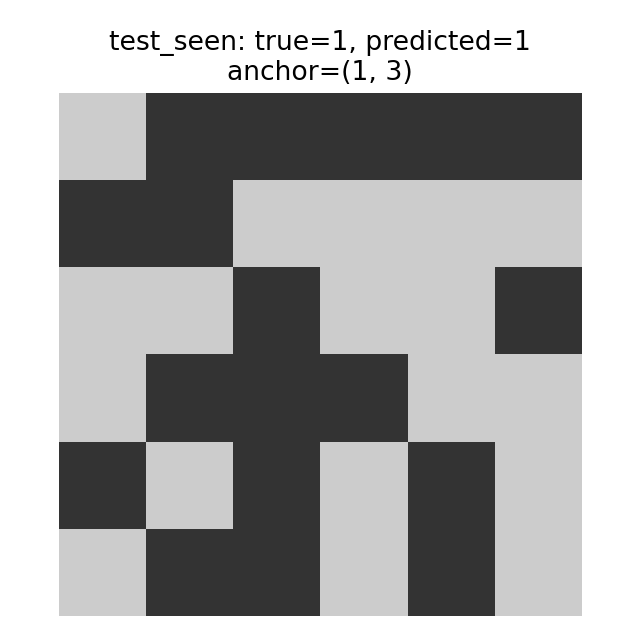
\includegraphics[width=0.24\linewidth]{q2_2_4_seen_1.png}\hfill
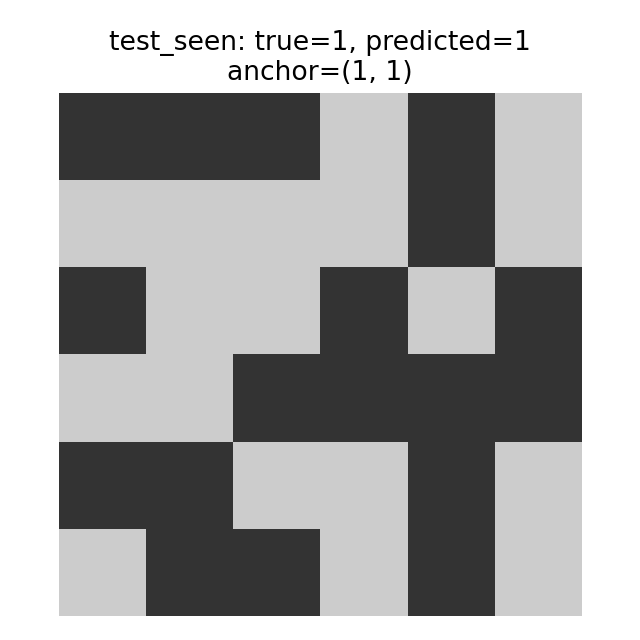
\includegraphics[width=0.24\linewidth]{q2_2_4_seen_4.png}\hfill
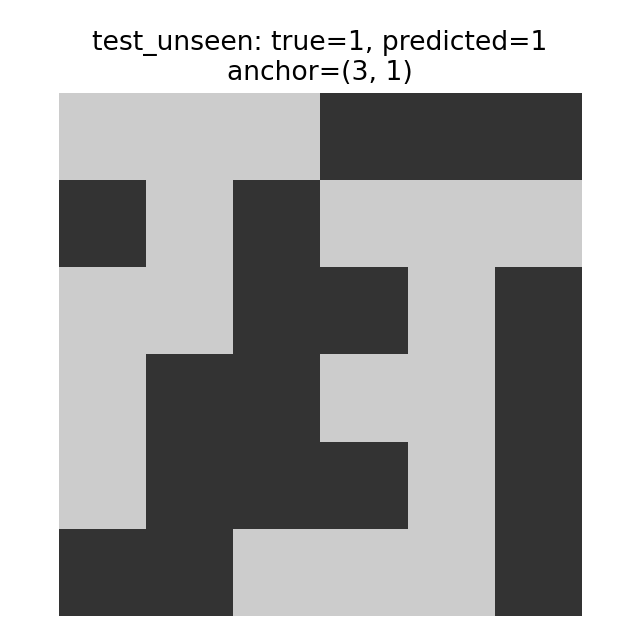
\includegraphics[width=0.24\linewidth]{q2_2_4_unseen_0.png}\hfill
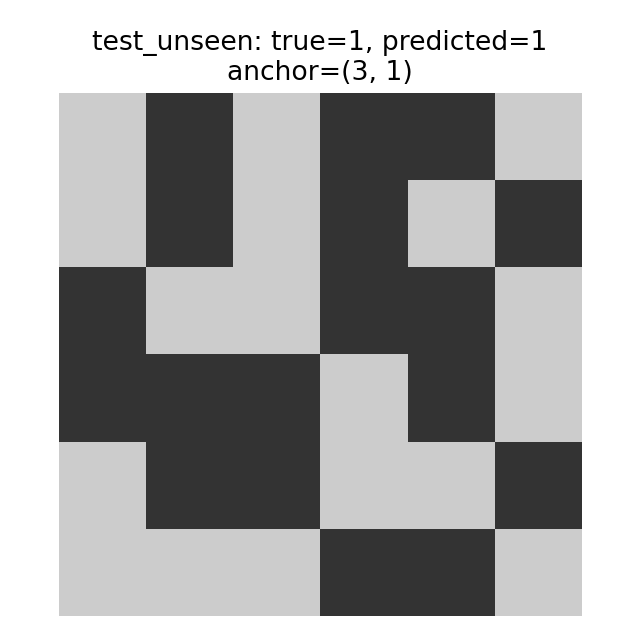
\includegraphics[width=0.24\linewidth]{q2_2_4_unseen_1.png}\par\smallskip
{\small\refstepcounter{qfig}\label{fig:q2-examples}\textbf{Figure~\theqfig.} Two positive examples from the seen-location test set (left) and two from the unseen-location test set (right), in the order of the table.\par}
\end{minipage}\par\medskip

No error occurred: all 512 images of each test set are classified correctly (confusion matrices above), so there is no misclassified example to discuss, and accuracy and recall are the same on seen and unseen locations. This agrees with the architecture: each convolution sees only a small neighbourhood (the receptive field of the second one is $8\times8$ pixels, the size of a $2\times2$ tile block), the same filters are applied at every position (weight sharing), and global max pooling keeps the strongest response of each channel wherever it occurs, so the features given to the linear layer depend mostly on whether a block is present and not on where it is.

This is empirical generalization of one trained model to two new locations, not guaranteed translation invariance. Zero padding treats the borders differently from the interior, and stride-2 pooling is only exactly equivariant to shifts that are multiples of 2 pixels (the shift between the seen and unseen rows, 8 pixels, is one). The unseen test images are also independently sampled boards rather than translated copies of seen ones, so the comparison is not a controlled translation test.

\end{enumerate}
}

\section*{Sources and assistance}
% Credit actual sources/tools and state their scope accurately, as required
% by the course policy. A declaration does not override restrictions on use.
   I used an AI assistant (Claude, through a coding-agent tool) for this assignment. Its role was:
   \begin{itemize}[leftmargin=*, itemsep=2pt, topsep=2pt]
   \item \textbf{Report:} it created the LaTeX skeleton, filled the tables from my notebook outputs
 and from \texttt{results.csv}, generated the figures (so they fill in the designed spaces without overflowing),
  and corrected the typos as well as the presentation of the results and discussion.
   \item \textbf{Analysis:} it explained course concepts that I used to form the expectations.
   \end{itemize}
   I ran all experiments myself, and every reported number comes from my notebook outputs.

\end{document}
